\documentclass[12pt,a4paper]{article}
\usepackage{fancyhdr}
\usepackage{fontspec}
\usepackage{amsmath}
\usepackage{amssymb}
\usepackage{bm}
\usepackage{tikz}
\usepackage{pstricks-add}
\setmainfont{Microsoft YaHei}
\pagestyle{fancy}


\begin{document}

\fancyfoot[C]{by chinasjtu@msn.com }

\newcommand{\nl}{\newline}

\newcommand{\ntinf}{\lim\limits_{n \to \infty}}
\newcommand{\xtinf}{\lim\limits_{x \to \infty}}

\newcommand{\Atinf}{\lim\limits_{A \to \infty}}
\newcommand{\Rtinf}{\lim\limits_{R \to \infty}}

\newcommand{\ntx}[1]{\lim\limits_{n \to #1}}
\newcommand{\xtx}[1]{\lim\limits_{x \to #1}}
\newcommand{\ttx}[1]{\lim\limits_{t \to #1}} 
\newcommand{\ktx}[1]{\lim\limits_{k \to #1}} 
\newcommand{\dxtx}[1]{\lim\limits_{\Delta x \to #1}}

\newcommand{\jfab}{\int_{a}^{b}}
\newcommand{\jf}[2]{\int_{#1}^{#2}}

\newcommand{\nsum}[2]{\sum\limits_{n=#1}^{#2}}
\newcommand{\isum}[2]{\sum\limits_{i=#1}^{#2}}
\newcommand{\ksum}[2]{\sum\limits_{k=#1}^{#2}}

\newcommand{\nsuminf} {\nsum{1}{\infty}}
\newcommand{\ksuminf} {\ksum{1}{\infty}}
\newcommand{\isuminf} {\isum{1}{\infty}}



$\nl$

\begin{center}第4章 导数与微分  \end{center}




$1^\circ \ f'(x_0)=\xtx{x_0}\frac{f(x)-f(x_0)}{x-x_0}$

$2^\circ \ \Delta y=f'(x_0)\Delta x+o(\Delta x),可导必连续$

$\\$

设f(x)在x=a处可导

$\ttx{0}\frac{f(a+t)-f(a-2t)}{2t}=\ttx{0}\frac{f(a+t)-f(a)-[f(a-2t)-f(a)]}{2t}$

$=\ttx{0}\frac{f(a+t)-f(a)}{2t}+\ttx{0}\frac{f(a-2t)-f(a)}{-2t}$

$=\frac{3}{2}f'(a) (逆命题未必成立)$


$\nl$
$例:设f(x)=|x-a|\cdot \varphi(x),其中\varphi(x)为连续函数,求f'_-(a),f'_+(a)$

问f(x)在x=a处可导条件

$\frac{\Delta y}{\Delta x}=\frac{f(a+\Delta x)-f(a)}{\Delta x} = \frac{|\Delta x|\varphi(a+\Delta x)}{\Delta x}$

$=\mp \varphi(a+\Delta x),\Delta x \lessgtr 0$

$f'_-(a) = -\varphi(a),f'_+(a) = +\varphi(a),当仅当\varphi(a)=0时可导$

$\nl$
定理2:
$设f(x)在x_0处左右导数均存在,则f(x_0)在x_0处必连续$

证明:
$\lim\limits_{\Delta x \to 0-}[f(x_0+\Delta x)-f(x_0)]=\lim\limits_{\Delta x \to 0-}\frac{[f(x_0+\Delta x)-f(x_0)]}{\Delta x} \Delta x$

$=f'-(x_0)·0=0,故左连续,同理可证右连续$

$\nl$
复合函数(链式法则),对数法则

$ex.1. y=\frac{(x+5)^2}{(x+2)^3}$

$lny=2ln(x+5)-3ln(x+2)$

$\frac{y'}{y}=\frac{2}{x+5}-\frac{3}{x+2}$

$y'=\frac{(x+5)^2}{(x+2)^3}(\frac{2}{x+5}-\frac{3}{x+2})$

$ex.2.y=x+x^x+x^{x^x}$

$y'=1+x^x(1+lnx)+...$

$\nl$

$\lim\limits_{\Delta x \to 0}\frac{\Delta y}{\Delta x}=\frac{dy}{dx},\frac{\Delta y}{\Delta x}=\frac{dy}{dx}+o(x)$

$\\$
$\S 4.3.微分$

一、微分概念

$定义:y=f(x),x\in U(x_0),若\exists A \in R(A为x之函数?)$

$\Delta y = f(x_0+\Delta x)-f(x_0)=A·\Delta x+o(\Delta x)$

$称f(x)在x_0可微,A\Delta x为f(x)在x_0处微分,记为dy|_{x=x_0},df|_{x=x_0}$

几何意义,在$(x_0,y_0)$处切线纵坐标改变量

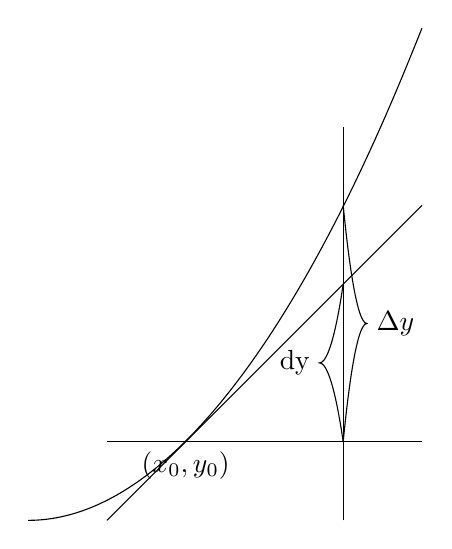
\begin{tikzpicture}
\draw (1,1) -- (5,1);
\draw (1,0) -- (5,4);
\draw (4,0) -- (4,5);
\draw (0,0) parabola (5,6.25);
\node [below] at (2,1) {$(x_0,y_0)$};
\node [left] at (3.7,2) {dy};
\draw (4,1) parabola bend (3.7,2) (4,3);
\node [right] at (4.3,2.5) {$\Delta y$};
\draw (4,1) parabola bend (4.3,2.5) (4,4);

\end{tikzpicture}

$\\$
$\nl$
高阶导数,高阶微分,P162

$dx^k=(dx)^k,d^kx表示对x的k次微分$

$\nl$
$f(x)在x_0处n阶可导 \to f^{n-1}(x)在x_0处连续 \to f^{n-k}(x) \in C(U(x_0)),k=2,3,4...n$

$\nl$
Ex.
$y=\frac{lnx}{x},y^n=\frac{(-1)^nn!}{x^{n+1}}[lnx-(1+\frac{1}{2}+\frac{1}{3}+...\frac{1}{n})]$

$\nl$
分段点处求导用定义

$\nl$
Ex.$y=arctg(x),求y^n(x)$

$y^1(-x^2+1)=1,同时求n-1阶导数(也可以看成y'=\frac{1}{2i}(\frac{1}{x-i}-\frac{1}{x+i}))$

$y'=\frac{1}{2i}(\frac{1}{x-i}-\frac{1}{x+i})$

$c_{n-1}^0(y')^{(n-1)}(1+x^2)^{(0)}+c_{n-1}^1(y')^{(n-2)}(1+x^2)^{(1)}+c_{n-1}^2(y')^{(n-3)}(1+x^2)^{(2)}$

$y^{(n)}(1+x^2)+(n-1)y^{(n-1)}2x+c_{n-1}^2y^{(n-2)}2=0$

$x=0代入,y_{(0)}^{(n)}=-(n-1)(n-2)y^{(n-2)}(0) \gets 递推公式$

$n=2k时,f^{(2k)}(0)=0$

$n=2k+1时,f^{(2k+1)}(0)=(2k)!(-1)^k$

$\nl$
隐函数P152

$\begin{cases}
x=a(cost+t·sint) \\
y=a(sint-t·cost)
\end{cases}$
$\frac{dy}{dx}=tgt$

$\nl$
极坐标

$r=r(\theta)$
$\begin{cases}
x=r(\theta)cos\theta \\
y=r(\theta)sin\theta
\end{cases}$

$\frac{dy}{dx}=\frac{r'(\theta)tg\theta+r(\theta)}{r'(\theta)-r'(\theta)tg\theta}$

$\newline$

$设ABC为平面三角形,l为已知直线,证明必存在平行l直线平分三角形面积$

$根据l方向建立坐标系(介值定理)$

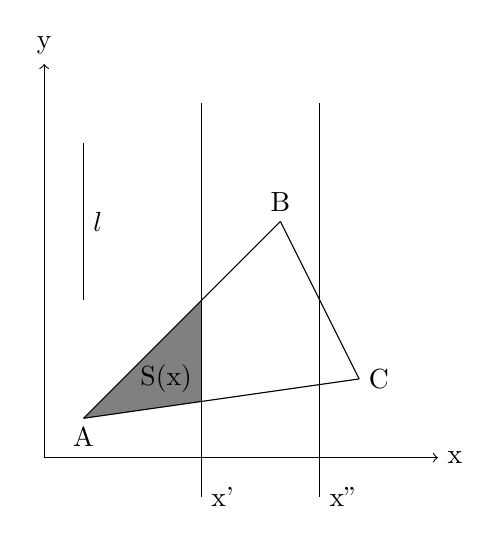
\begin{tikzpicture}
\fill[gray] (0.5,0.5) -- (2,0.714) -- (2,2);
\draw[->] (0,0) -- (5,0);
\draw[->] (0,0) -- (0,5);
\node [right] at (5,0) {x};
\node [above] at (0,5) {y};
\draw (0.5,0.5) -- (4,1);
\draw (0.5,0.5) -- (3,3);
\draw (3,3) -- (4,1);
\draw (0.5,2) -- (0.5,4);
\node [right] at (0.5,3) {$l$};
\node [right] at (4,1) {C};
\node [above] at (3,3) {B};
\node [below] at (0.5,0.5) {A};
\draw (3.5,-0.5) -- (3.5,4.5);
\node [right] at (3.5,-0.5) {x''};
\draw (2,-0.5) -- (2,4.5);
\node [right] at (2,-0.5) {x'};
\node [left] at (2,1) {S(x)};
\end{tikzpicture}

$A,B,C,(x_1,x_2,x_3)$

$x_1<x_2<x_3$

定义左侧面积为S(x)

$|S(x)-S(x'')| \le |x''-x|·max(y_1,y_2,y_3)$

故S(x)为一致连续函数

$\nl$

平面上有n个点,证明必存在一面积最小的圆,将此n个点全部盖住,且此圆唯一

证明:唯一性(易证,如下所示两圆交集)。

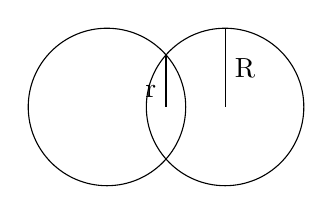
\begin{tikzpicture}
\draw (0,0) circle (1);
\draw (1.5,0) circle (1);
\draw (1.5,0) -- (1.5,1);
\draw (0.75,0) -- (0.75,0.66);
\node [right] at (1.5,0.5) {R};
\node [left] at (0.75,0.2) {r};
\end{tikzpicture}

有R,则有r<R,矛盾。

存在性,确界定理。

$\nl$

设f(x)在[a,b]上定义,若f(x)每个值恰好取两次,证明f(x)在[a,b]不连续

假设连续,则可取最大值,最小值2次

\begin{tikzpicture}
\draw (1,0) -- (8.5,0);
\draw (2,-1) -- (2,5);
\draw (4,0) -- (4,4);
\draw (7,0) -- (7,4);
\node [above] at (4,4) {$最大$};
\node [above] at (7,4) {$最大$};
\node [below] at (4,0) {A};
\node [below] at (7,0) {B};
\draw (6.5,0) -- (6.5,3.7);
\node [below] at (6.5,0) {$x_3$};

\draw (5,0) -- (5,3);
\draw (3.3,3) -- (5,3);
\draw (3.3,3) -- (3.3,0);
\node [below] at (5,0) {$x_2$};
\node [below] at (3.3,0) {$x_1$};

\draw (3,2) parabola bend (4,4) (5,3);
\draw (5,3) parabola bend (5.5,2.5) (6,3);
\draw (6,3) parabola bend (7,4) (8,3);

\draw (3,2) -- (3,0);
\node [below] at (3,0) {a};
\draw (8,3) -- (8,0);
\node [below] at (8,0) {b};
\end{tikzpicture}

$设f(x_3)>f(x_1),f(x_3)>f(x_2)$

$则x_1与A,A与x_2之间有与f(x_3)相同的值存在,矛盾$

$\nl$

$设f(x)在R上一致连续,证明必存在A,B>0,使得|f(x)|\le A|x|+B$

证明:$取\varepsilon_0=1,由f(x)\in U(R),故有\exists \delta >0,|f(x_1)-f(x_2)|<\varepsilon_0=1,\forall x_1,x_2 \in R,|x_1-x_2|<\delta$

$\forall x \in R,|x|\le \delta,取n=[\frac{|x|}{\delta}]+1$

$由\frac{|x|}{\delta}<n\le\frac{|x|}{\delta}+1 \to \frac{|x|}{n}<\delta\le\frac{|x|}{n-1}$

$于是|f(x)-f(0)|\le|f(x)-f(\frac{n-1}{n}x)|+|f(\frac{n-1}{n}x)-f(\frac{n-2}{n}x)|+...+|f(\frac{1}{n}x)-f(0)|<n·\varepsilon_0=n$

故有$|f(x)|<|f(0)|+n\le|f(0)|+\frac{|x|}{\delta}+1$

$若|x|<\delta,|f(x)|<|f(0)|+1\le|f(0)|+\frac{|x|}{\delta}+1$

取$A=\frac{1}{\delta},B=|f(0)|+1,\delta 是对于\varepsilon_0 取1时而有的 $

$\nl$

\begin{tikzpicture}
\draw (0,0) rectangle (3,2);
\draw (6,0) rectangle (9,2);
\draw (12,0) rectangle (15,2);

\node at (1.5,1) {无穷大};
\node at (7.5,1) {无界};
\node at (13.5,1) {无极限};

\draw (0,4) rectangle (3,6);
\draw (6,4) rectangle (9,6);
\draw (12,4) rectangle (15,6);

\node at (1.5,5) {无穷小};
\node at (7.5,5) {有极限};
\node at (13.5,5) {有界};

\draw[<->] (1.5,2) -- (1.5,4);
\node at (1.5,3) {互为倒数};

\draw[<->] (13.5,2) -- (13.5,4);
\node at (13.5,3) {反例};


\draw[->] (3,1.5) -- (6,1.5);
\node at (4.5,1.5) {可证};

\draw[->] (9,1.5) -- (12,1.5);
\node at (10.5,1.5) {可证};

\draw[->] (3,5.5) -- (6,5.5);
\node at (4.5,5.5) {可证};

\draw[->] (9,5.5) -- (12,5.5);
\node at (10.5,5.5) {可证};

\draw[<-] (3,0.5) -- (6,0.5);
\node at (4.5,0.5) {反例2};

\draw[<-] (9,0.5) -- (12,0.5);
\node at (10.5,0.5) {反例1};

\draw[<-] (3,4.5) -- (6,4.5);
\node at (4.5,4.5) {反例};

\draw[<-] (9,4.5) -- (12,4.5);
\node at (10.5,4.5) {反例1};

\end{tikzpicture}

反例1:0,1,0,1.....

反例2:x·sinx


无界数列中必有无穷大子列

$\nl$

隐函数与参数方程的高阶导数P168

$\nl$
习题课

$f(u)在u_0可导,u=g(x)在x_0不可导,f(g(x))在x_0处是否必不可导,反例u=|x|,f(u)=u^2$

$f(u)在u_0不可导,u=g(x)在x_0不可导,f(g(x))在x_0处是否必不可导,反例f=g=\frac{1}{x}$

$f(x)\ge g(x) 必有f'(x)\ge g'(x)? 反例:f=e^{-x},g=-e^{-x}$

$\nl$

$(\frac{1-x}{1+x})^{(n)}=\frac{2(-1)^nn!}{(1+x)^{n+1}}$

$\nl$
$f(x)在(a,b)内可导,\xtx{a+0}f(x)=\infty,是否必有\xtx{a+0}f'(x)=\infty$

反例$f(x)=\frac{1}{x}+cos\frac{1}{x},x\in(0,1)$

$f'(x)=-\frac{}1{x^2}(1+sin\frac{1}{x})$

逆命题反例$y=\sqrt{x}$

$y'=\frac{1}{2\sqrt x}$

$\nl$
$f(x)在[a,+\infty)上可导,\xtx{+\infty}f(x)存在,\xtx{+\infty}f'(x)也存在?$

反例$f(x)=\frac{sin(x^2)}{x}, x\in[1,+\infty)$

$\nl$
$f(x)为奇偶性具有的函数,f'(x)也具有奇偶性,但奇偶性改变(可证)$

$\nl$
$f(x)为具有周期性的函数,f'(x)也具有周期性(可证)$

$\nl$
$y=|x+1|^3-2,x \in R,求f'(x),f''(x)$

$
y'=\begin{cases}
3(x+1)^2, & x>-1 \\
0, & x=-1 \\
-3(x+1)^2, & x<-1
\end{cases}
$

$
y''=\begin{cases}
6(x+1), & x>-1 \\
0, & x=-1 \\
-6(x+1), & x<-1
\end{cases}
$

$f''(-1)用f'(x)的x=-1的左右导数来求,f''_{\pm}(-1)=0$

$f'''_{\pm}(-1)=\lim\limits_{\Delta x \to 0\pm}\frac{\pm 6 \Delta x-0}{\Delta x}=\pm 6$

$\nl$

$
f(x)=\begin{cases}
x^2e^{-x^2}, & |x|\le 1 \\
\frac{1}{e}, & |x|>1
\end{cases}
$

$
f'(x)=\begin{cases}
2xe^{-x^2}(1-x^2), & |x|\le 1 \\
0, & |x|>1
\end{cases}
$

$f'_+(1)=0,f'_-(0)=\xtx{1^-}\frac{x^2(e^{1-x^2}-1)+x^2-1}{e(x-1)}$

$=\xtx{1^-}[-x^2(1+x)\frac{e^{1-x^2}-1}{e(1-x^2)}+\frac{1+x}{e}]$

$=-\frac{2}{e}+\frac{2}{e}=0$

$\nl$
$例 \ 设f(x)在[a,b]上可导,且f'_+(a) \ne f'_-(b),则对\forall C$

$C介于f'_+(a)和f'_-(b)之间,则\exists x_0 \in (a,b),有$

$f'(x_0)=C \Leftrightarrow \exists (f(x)-Cx)'=0(导数介值定理,达布定理)$

$不妨设f'_+(a) < C < f'_-(b),构造F(x)=f(x)-Cx$

$则F(x)在[a,b]上可导,F(x)\in C[a,b]$

F(x)在[a,b]上有最大值和最小值

$记F(x_0)=\min F(x)$

由Fermat引理有$F'(x_0)=0 \Rightarrow f'(x_0)=C$

$若x_0=a或b,则F(a) \le F(x),\forall x \in U(a)$

则有$\frac{F(x)-F(a)}{x-a} \ge 0,F'(a)=f'_+(a)-C \ge 0$

$f'_+(a)\ge C 与条件矛盾$

\end{document}

